\section{Returns time series simulations}
\label{sec:simulations}

In Sect. \ref{subsec:gauss_alg_sim} we simulate returns time series following
a multivariate Gaussian and algebraic distribution. We test the influence of
the normalization within the epochs in the ergodicity defect in Sect.
\ref{subsec:norm_epochs_sim} and propose a solution for this defect in Sect.
\ref{subsec:norm_full_sim}. Finally we use empirical data to support our
simulation findings in Sect. \ref{subsec:emp_results}.

%%%%%%%%%%%%%%%%%%%%%%%%%%%%%%%%%%%%%%%%%%%%%%%%%%%%%%%%%%%%%%%%%%%%%%%%%%%%%%%
\subsection{Simulation of multivariate Gaussian and algebraic distributions}
\label{subsec:gauss_alg_sim}

In Sect. \ref{subsubsec:gauss_sim} we describe the methodology to simulate
multivariate Gaussian distributed returns time series and in Sect.
\ref{subsubsec:alg_sim} we describe the methodology to simulate multivariate
algebraic distributed returns time series.

%%%%%%%%%%%%%%%%%%%%%%%%%%%%%%%%%%%%%%%%%%%%%%%%%%%%%%%%%%%%%%%%%%%%%%%%%%%%%%%
\subsubsection{Multivariate Gaussian distributions}\label{subsubsec:gauss_sim}

To simulate the returns time series, we use a method \cite{drawing_dist} for
drawing a random vector $x$ from the $N$-dimensional multivariate Gaussian
distribution with mean vector $\mu$ and covariance matrix $\Sigma$. First, we
create a correlation matrix $C$ with $c = 1$ on its diagonal and $c = 0.3$ on
its non-diagonal entries. Then, we compute the eigenvalues and eigenvectors of
the correlation matrix, such that $C = U \Lambda U^{-1}$. We get a $z$ vector
whose components are drawn from a independent standard Gaussian distribution.
Finally we obtain the returns with the desired distribution as
\begin{equation}
    r = \mu + U \Lambda^{1/2} z
\end{equation}

In our case, the $r$ vector components are drawn from a normal distribution
with $\mu$ vector zero.
With these method we want to obtain time series simulating the data matrix G
with dimensions $2 \times T$, where $T$ is the window length of the epochs.
These returns can be later normalized, rotated and aggregated to compare with
the behavior of the results in Sect. \ref{subsec:epochs}.  The goal of this
approach is that all simulations should show standard normal distributions.

\begin{figure}[htbp]
    \centering
    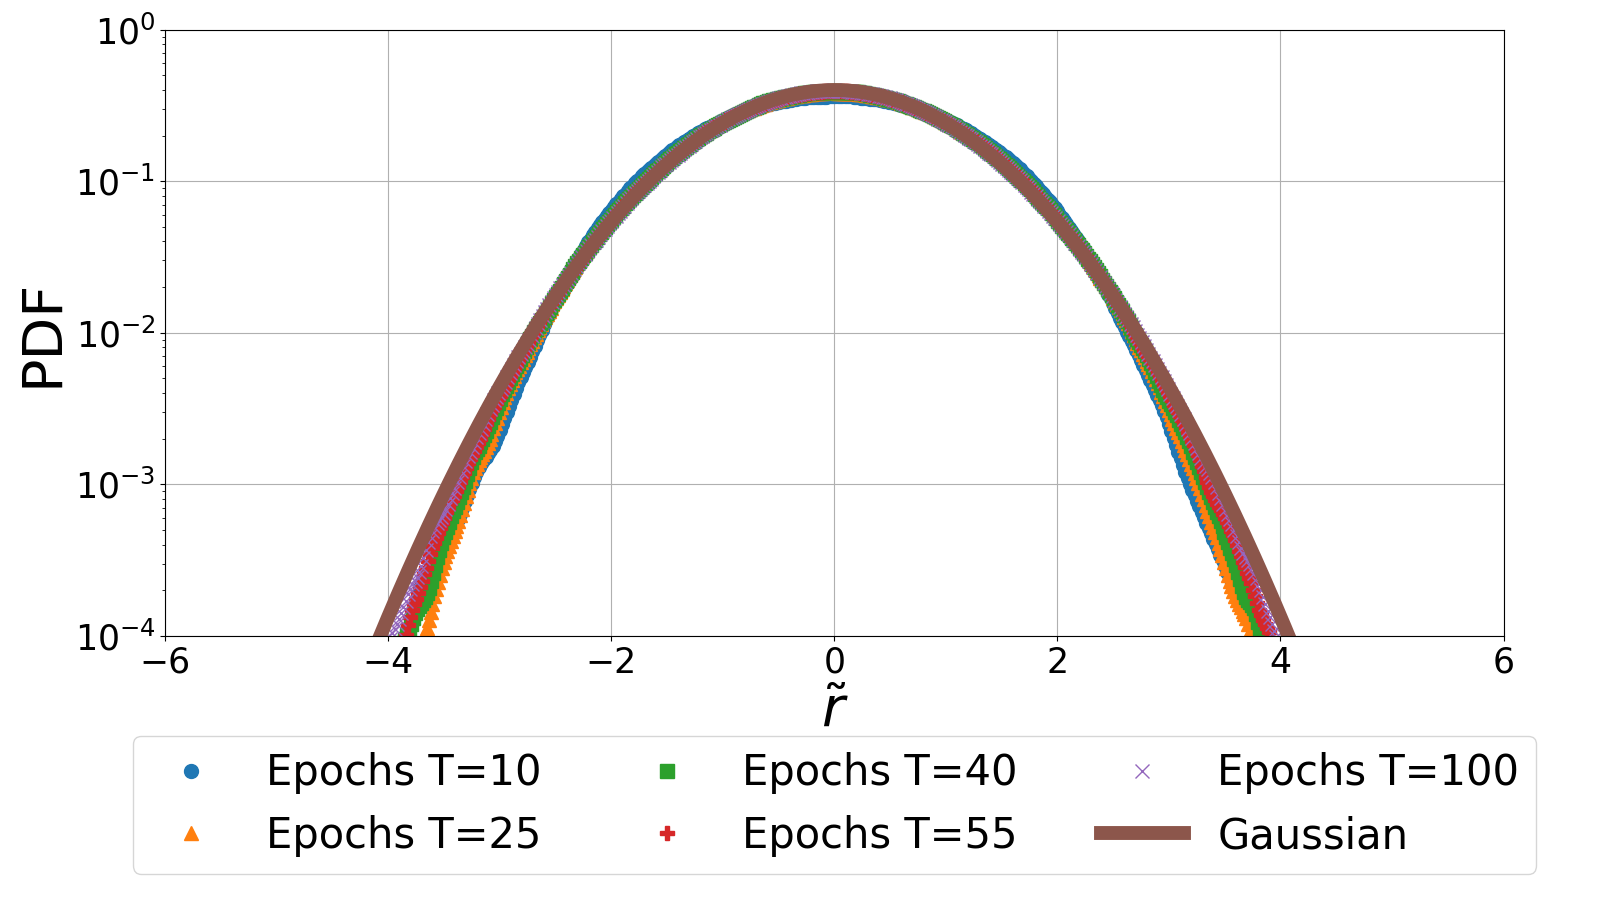
\includegraphics[width=0.6\columnwidth]
    {figures/06_epochs_sim_gauss_agg_ret_pairs_no_norm.png}
    \caption{Simulated aggregated rotated and scaled Gaussian distributed
             returns ($\tilde{r}$) for fixed covariance and $K=200$ without
             normalization, neither within the epochs nor for all the time
             series. $\Delta t = 1$ unit and epochs window  lengths
             $T=10, 25, 40, 55, 100$ units.}
    \label{fig:gauss_epochs_agg_ret_pairs_no_norm}
\end{figure}

In Fig. \ref{fig:gauss_epochs_agg_ret_pairs_no_norm} we simulate time series
for $K = 200$. Each time series is made of $200$ epochs to make them comparable
to the empirical data. We use epochs window lengths $T = 10, 25, 40, 55$ units
to rotate, scale and aggregate without normalizing neither within the epochs
nor the full time series. As expected, as we draw the returns from a
multivariate Gaussian distribution, all the simulations show standard Gaussian
distribution behavior. Thus, this is our reference to check what is introducing
the ergodicity defect in the original method for the multivariate Gaussian
case.

%%%%%%%%%%%%%%%%%%%%%%%%%%%%%%%%%%%%%%%%%%%%%%%%%%%%%%%%%%%%%%%%%%%%%%%%%%%%%%%
\subsubsection{Multivariate algebraic distributions}\label{subsubsec:alg_sim}

To simulate returns time series drawn from multivariate algebraic
distributions, we use a similar approach as in Sect. \ref{subsubsec:gauss_sim}.
First, we create a correlation matrix $C$ with $c = 1$ on its diagonal and
$c = 0.3$ on its non-diagonal entries. From \cite{t_student_dist} we know that
\begin{equation}
    T = \left( S^{-1/2} \right)^{\dagger} X + M,
\end{equation}
where $T$ is a vector of length $K$. Then it is needed to repeat the following
steps to generate a data matrix where the columns are the $T$ vectors. $X$ is
drawn from a matrix variate normal distribution. Matrix $S$ is a Wishart
distributed covariance matrix without normalization and M is a parameter that
for this case is zero. With these in mind, we first generate $S$ as a
positive semi-definite matrix. To do this, we first create time series of
simulated data matrix $G$ with dimension $K \times \left(n + K - 1 \right)$
where $n$ is the a parameter of the degree of freedom and is connected to the
shape parameter $l$ as
\begin{equation}
    l = \frac{n + K}{2},
\end{equation}
where $K$ is the number of companies. These time series are generated by
calculating
\begin{equation}
    y = U \Lambda^{1/2} z
\end{equation}
with a fixed covariance matrix $\Sigma$. Vector $y$ is a column vector of $G$,
$z$ is a univariate standard normal distribution vector, $U$ has the
eigenvectors of $\Sigma$ as columns and the diagonal matrix $\Lambda$ contains
the eigenvalues of $\Sigma$. Thus, we compute
\begin{equation}
    S = G G^{\dagger}
\end{equation}
Then, we obtain $S^{1/2}$ as
\begin{equation}
    S^{1/2} = U_{S} \Lambda_{S}^{1/2} U_{S}^{\dagger},
\end{equation}
since
\begin{align}
    S &= S^{1/2} S^{1/2} \\
    &= U_{S} \Lambda_{S}^{1/2} U_{S}^{\dagger}
    U_{S} \Lambda_{S}^{1/2} U_{S}^{\dagger}\\
    &= U_{S} \Lambda_{S} U_{S}^{\dagger}
\end{align}
We generate $X$ as
\begin{equation}
    X = \sqrt{m} z
\end{equation}
where $z$ is a univariate standard normal distribution vector of length $K$ and
$m$ is the variance.

These returns can be later normalized, rotated and aggregated to compare with
the behavior of the results in Sect. \ref{subsec:epochs}.  The goal of this
approach is that all simulations should show standard algebraic distributions.

\begin{figure}[htbp]
    \centering
    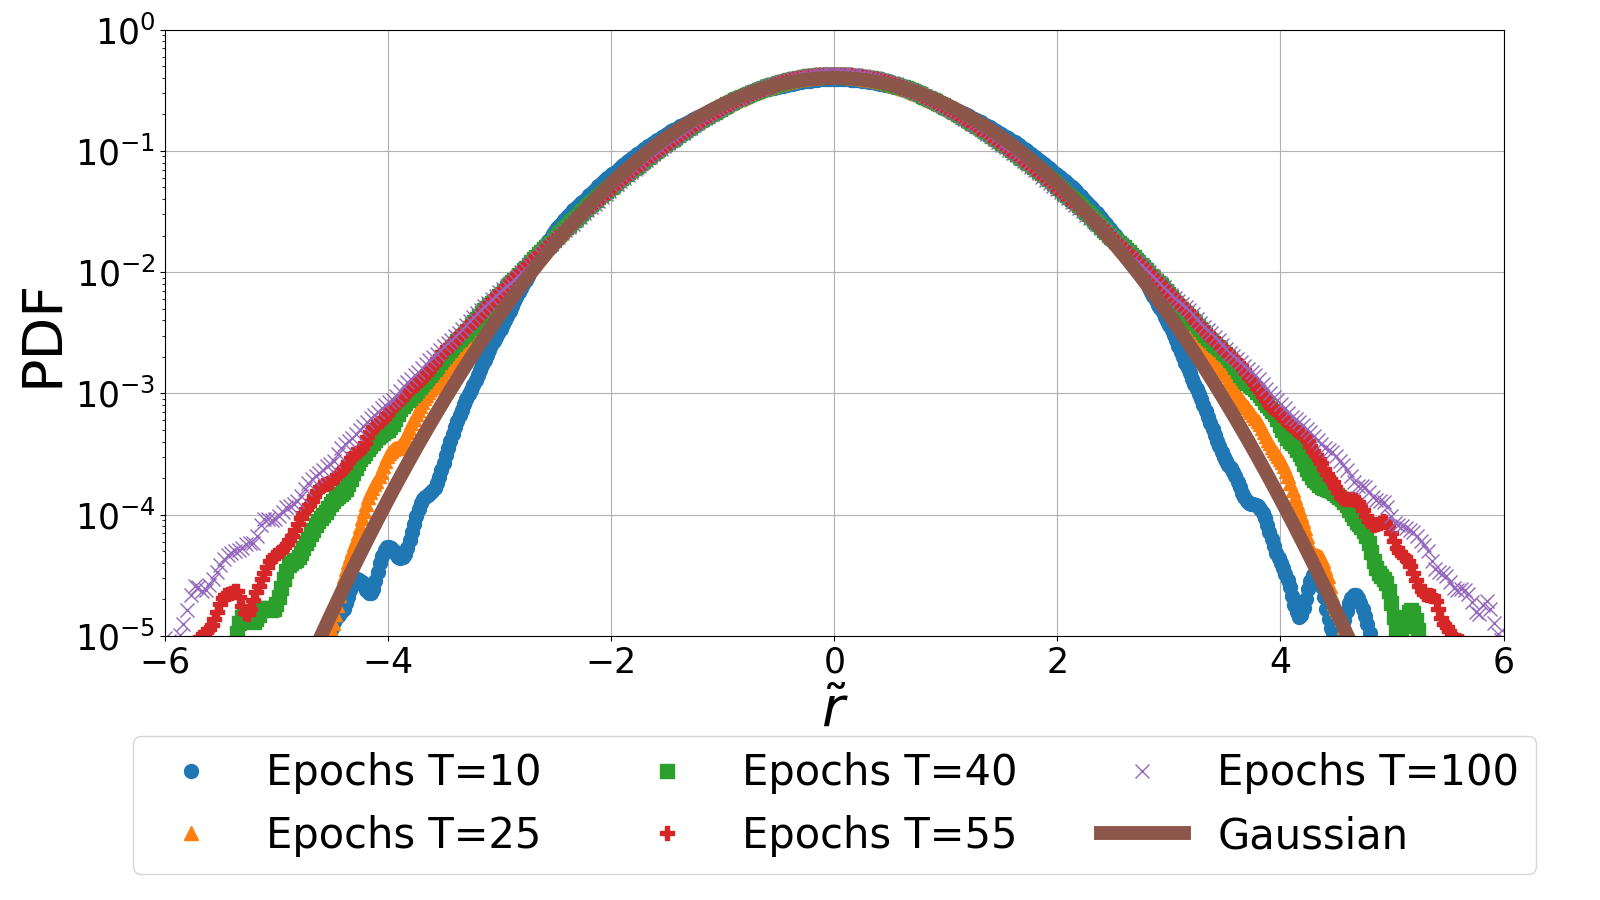
\includegraphics[width=0.6\columnwidth]
    {figures/06_epochs_sim_alg_agg_ret_pairs_no_norm.png}
    \caption{Simulated aggregated rotated and scaled algebraic distributed
             returns ($\tilde{r}$) for fixed covariance and $K=200$ without
             normalization, neither within the epochs nor for all the time
             series. $\Delta t = 1$ unit and epochs window  lengths
             $T=10, 25, 40, 55, 100$ units.}
    \label{fig:alg_epochs_agg_ret_pairs_no_norm}
\end{figure}

In Fig. \ref{fig:alg_epochs_agg_ret_pairs_no_norm} we simulate time series for
$K = 200$. Each time series is made of $200$ epochs to make them comparable
to the empirical data. We use epochs window lengths $T = 10, 25, 40, 55$ units
to rotate, scale and aggregate without normalizing neither within the epochs
nor the full time series. We can see an interesting behavior in the algebraic
case, where for small epochs window lengths, the tails are similar to the
Gaussian distribution, and as the epochs window lengths grow, the simulations
reveals good agreement with the algebraic distribution. Thus, this is our
reference to check what is introducing the ergodicity effect in the original
method for the multivariate algebraic case.

%%%%%%%%%%%%%%%%%%%%%%%%%%%%%%%%%%%%%%%%%%%%%%%%%%%%%%%%%%%%%%%%%%%%%%%%%%%%%%%
\subsection{Normalization within the epochs}
\label{subsec:norm_epochs_sim}

Now, to check the normalization within the epochs, we first simulate the
returns and then normalize each epoch to mean $\mu = 0$ and variance
$\sigma^{2} = 1$. Finally we repeat the procedure of rotate, scale and
aggregate.

For the Gaussian case with the simulated pair returns time series, we proceed
to normalize the epoch, compute the $2 \times 2$ sample covariance matrix and
diagonalize it. We rotate the two-component returns vectors into the eigenbasis
of the covariance matrix and normalize the axis with the eigenvalues. Finally
we aggregate all the components into a single univariate distribution.

\begin{figure}[htbp]
    \centering
    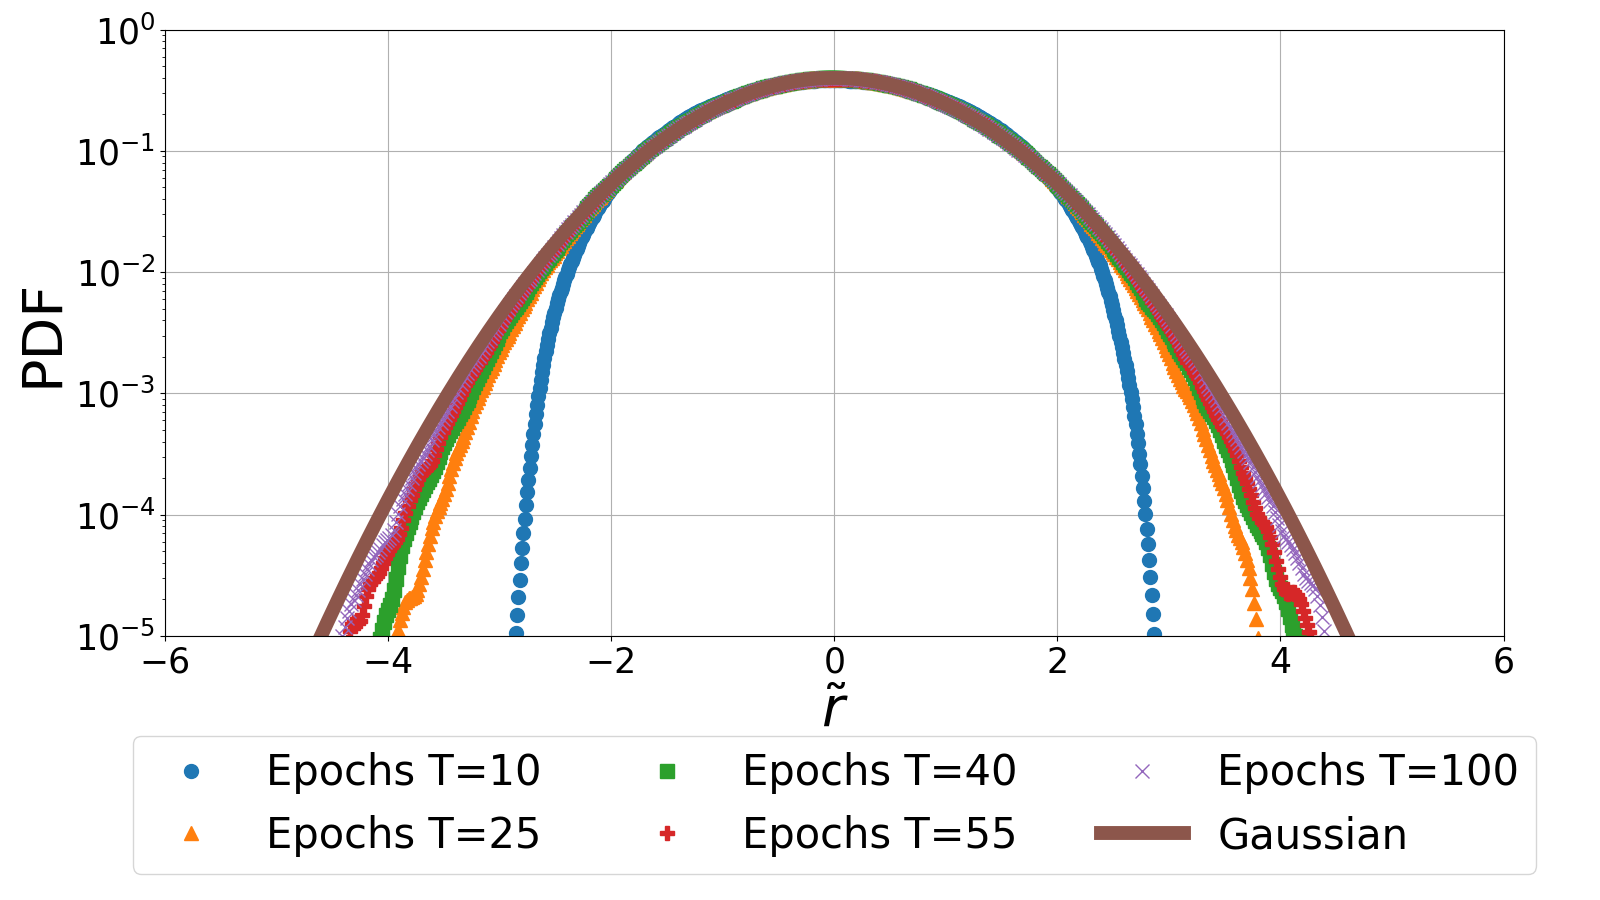
\includegraphics[width=0.6\columnwidth]
    {figures/06_epochs_sim_gauss_agg_ret_pairs_norm.png}
    \caption{Simulated aggregated rotated and scaled Gaussian distributed
             returns ($\tilde{r}$) for fixed covariance and $K=200$ with
             normalization within the epochs. $\Delta t = 1$ unit and epochs
             window lengths $T=10, 25, 40, 55, 100$ units.}
    \label{fig:epochs_gauss_agg_ret_pairs_norm}
\end{figure}

As we can see in Fig. \ref{fig:epochs_gauss_agg_ret_pairs_norm}, the ergodicity
defect clearly appears for an epoch window length $T = 10$. As the epoch window
length grows, the ergodicity defect starts to disappear. We could even argue,
that with an epoch window length greater or equal to $T = 25$, we already are
close enough to the Gaussian distribution. Thus, this ergodicity defect has a
large impact in small epochs window length, and its effects tends to disappear
as the epochs window lengths grow. This can be seen with $T = 100$.

Something similar happens with the algebraic case. We again simulate the
returns, normalize each epoch to mean $\mu = 0$ and variance $\sigma^{2} = 1$
and finally repeat the procedure of rotate, scale and aggregate. In Fig.
\ref{fig:epochs_alg_agg_ret_pairs_norm} can be seen how the ergodicity effect
appears again. It seems to have a large effect in epochs window lengths with
small values. Thus, we need to find an alternative to solve this problem.

\begin{figure}[htbp]
    \centering
    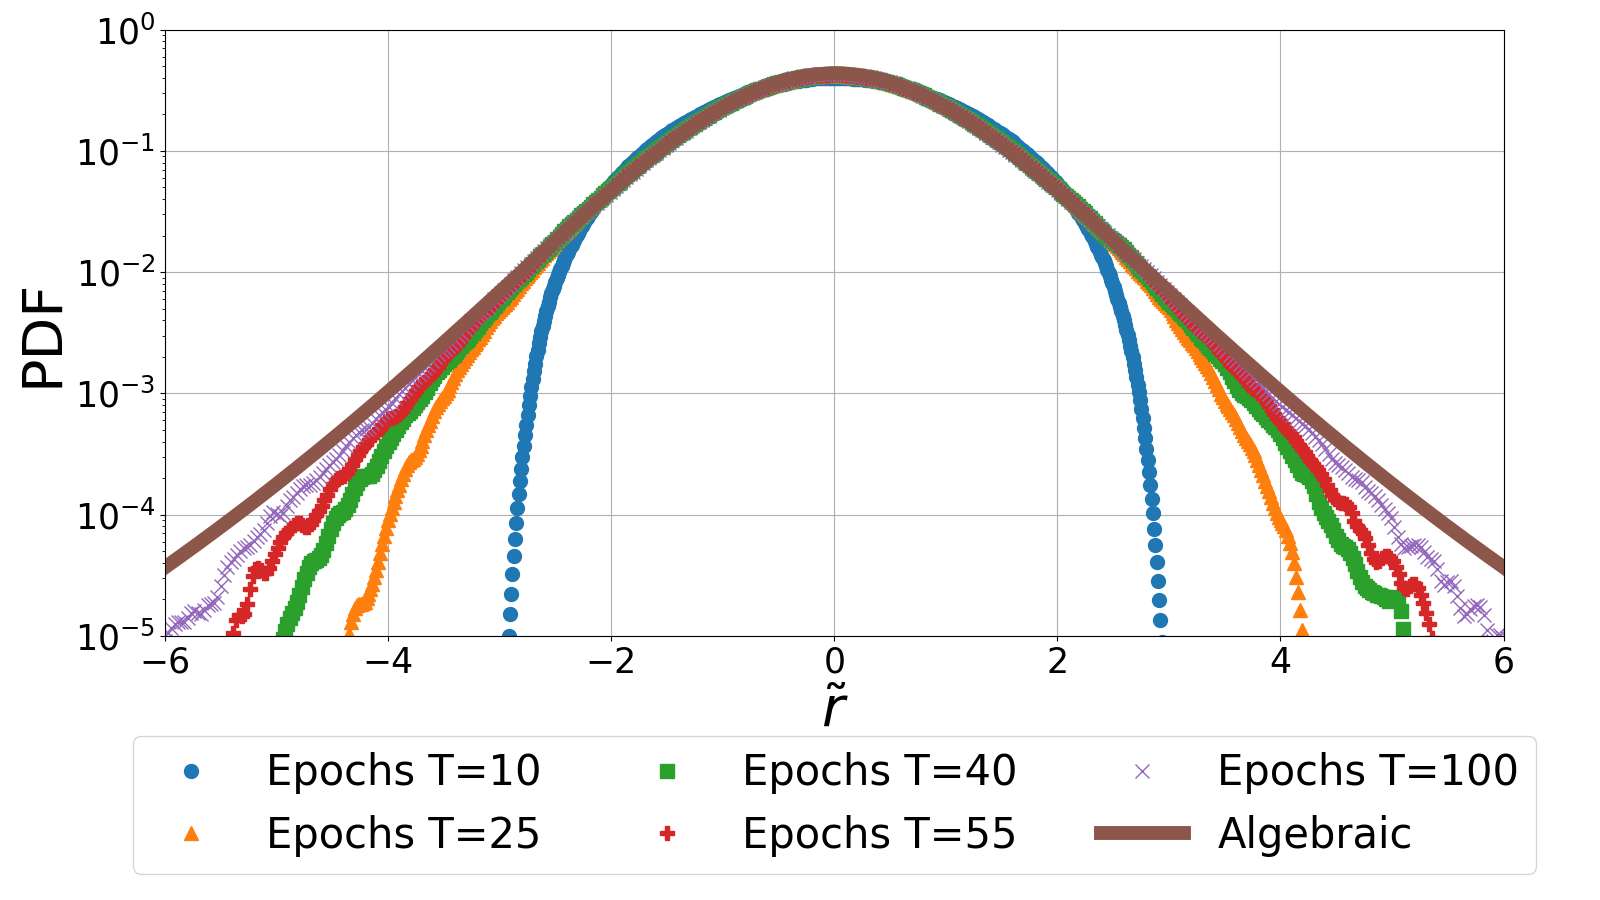
\includegraphics[width=0.6\columnwidth]
    {figures/06_epochs_sim_alg_agg_ret_pairs_norm.png}
    \caption{Simulated aggregated rotated and scaled Gaussian distributed
             returns ($\tilde{r}$) for fixed covariance and $K=200$ with
             normalization within the epochs. $\Delta t = 1$ unit and epochs
             window lengths $T=10, 25, 40, 55, 100$ units.}
    \label{fig:epochs_alg_agg_ret_pairs_norm}
\end{figure}

%%%%%%%%%%%%%%%%%%%%%%%%%%%%%%%%%%%%%%%%%%%%%%%%%%%%%%%%%%%%%%%%%%%%%%%%%%%%%%%
\subsection{Normalization complete return time series}
\label{subsec:norm_full_sim}

We already showed that the ergodicity defect is directly related with the
normalization of the time series. To try to solve this issue, instead of
normalizing the time series within each epoch, we normalize the complete time
series and then proceed to rotate, scale and aggregate.

In Fig. \ref{fig:epochs_gauss_agg_ret_pairs_norm_full_ts} and Fig.
\ref{fig:epochs_alg_agg_ret_pairs_norm_full_ts} are shown the Gaussian and
algebraic cases with the corresponding simulations. We can notice how in both
cases the ergodicity defect disappears. In each epochs window length, the
probability density function perfectly fits the Gaussian distribution and the
algebraic distribution. It can be noted that the larger the epochs window
length, the better the simulated data fit the distributions. Furthermore, to
accomplish our assumption of stationarity on short time scales, the results
for short epochs window lengths have a good agreement with the theoretical
distribution.

\begin{figure}[htbp]
    \centering
    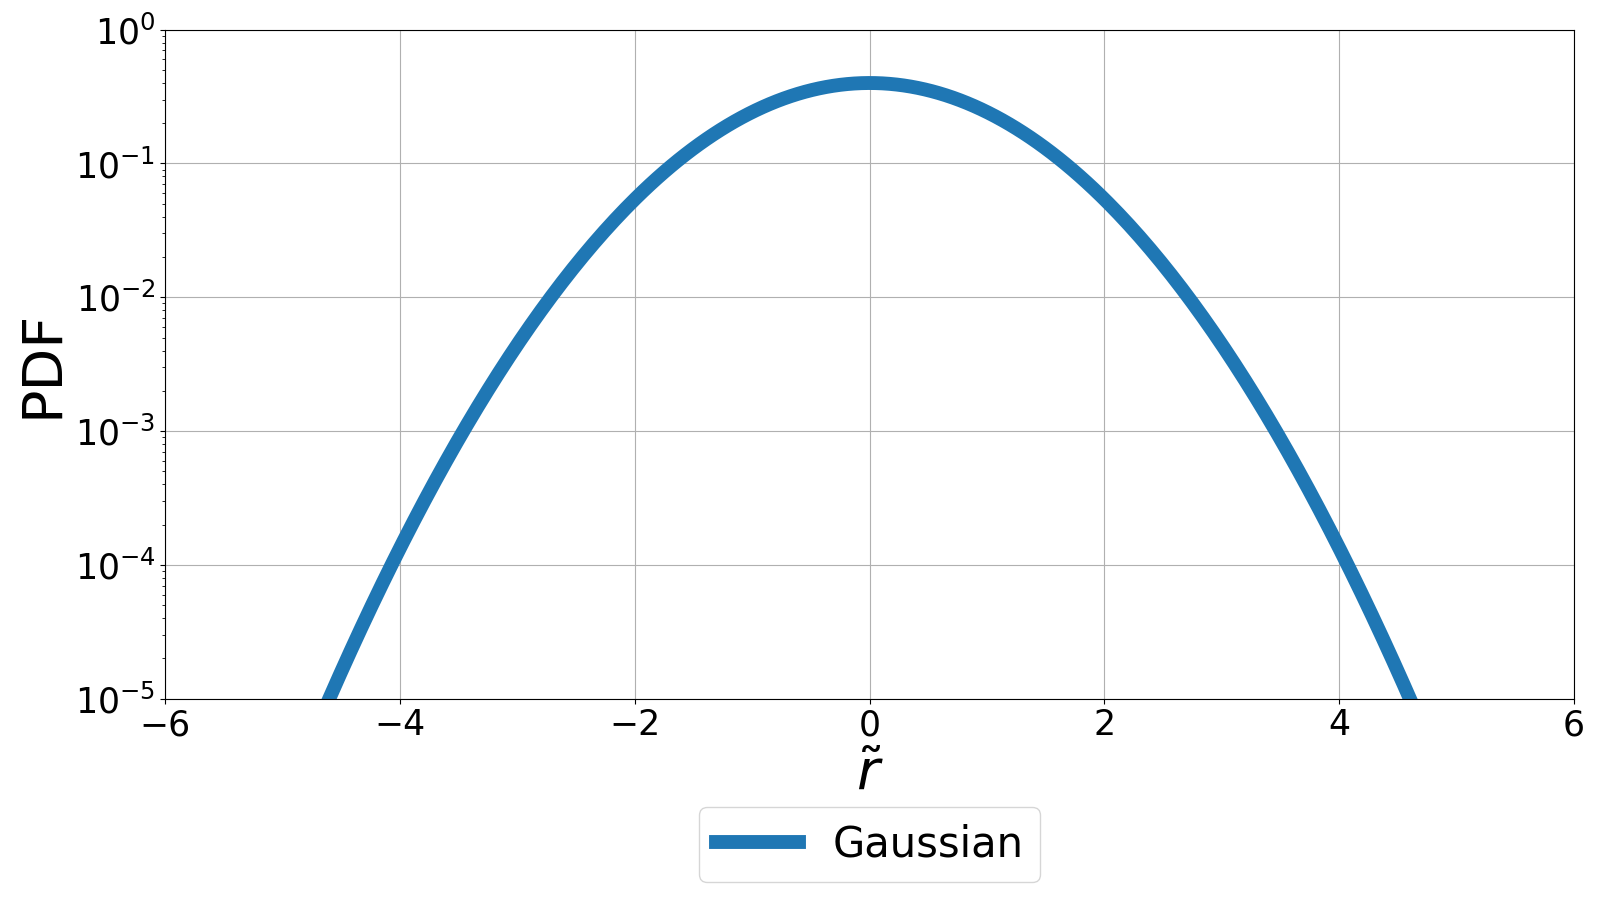
\includegraphics[width=0.6\columnwidth]
    {figures/06_epochs_sim_gauss_ts_norm.png}
    \caption{Simulated aggregated rotated and scaled Gaussian distributed
             returns ($\tilde{r}$) for fixed covariance and $K=200$ with
             normalization for the complete time series. $\Delta t = 1$ unit
             and epochs window lengths $T=10, 25, 40, 55, 100$ units.}
    \label{fig:epochs_gauss_agg_ret_pairs_norm_full_ts}
\end{figure}

\begin{figure}[htbp]
    \centering
    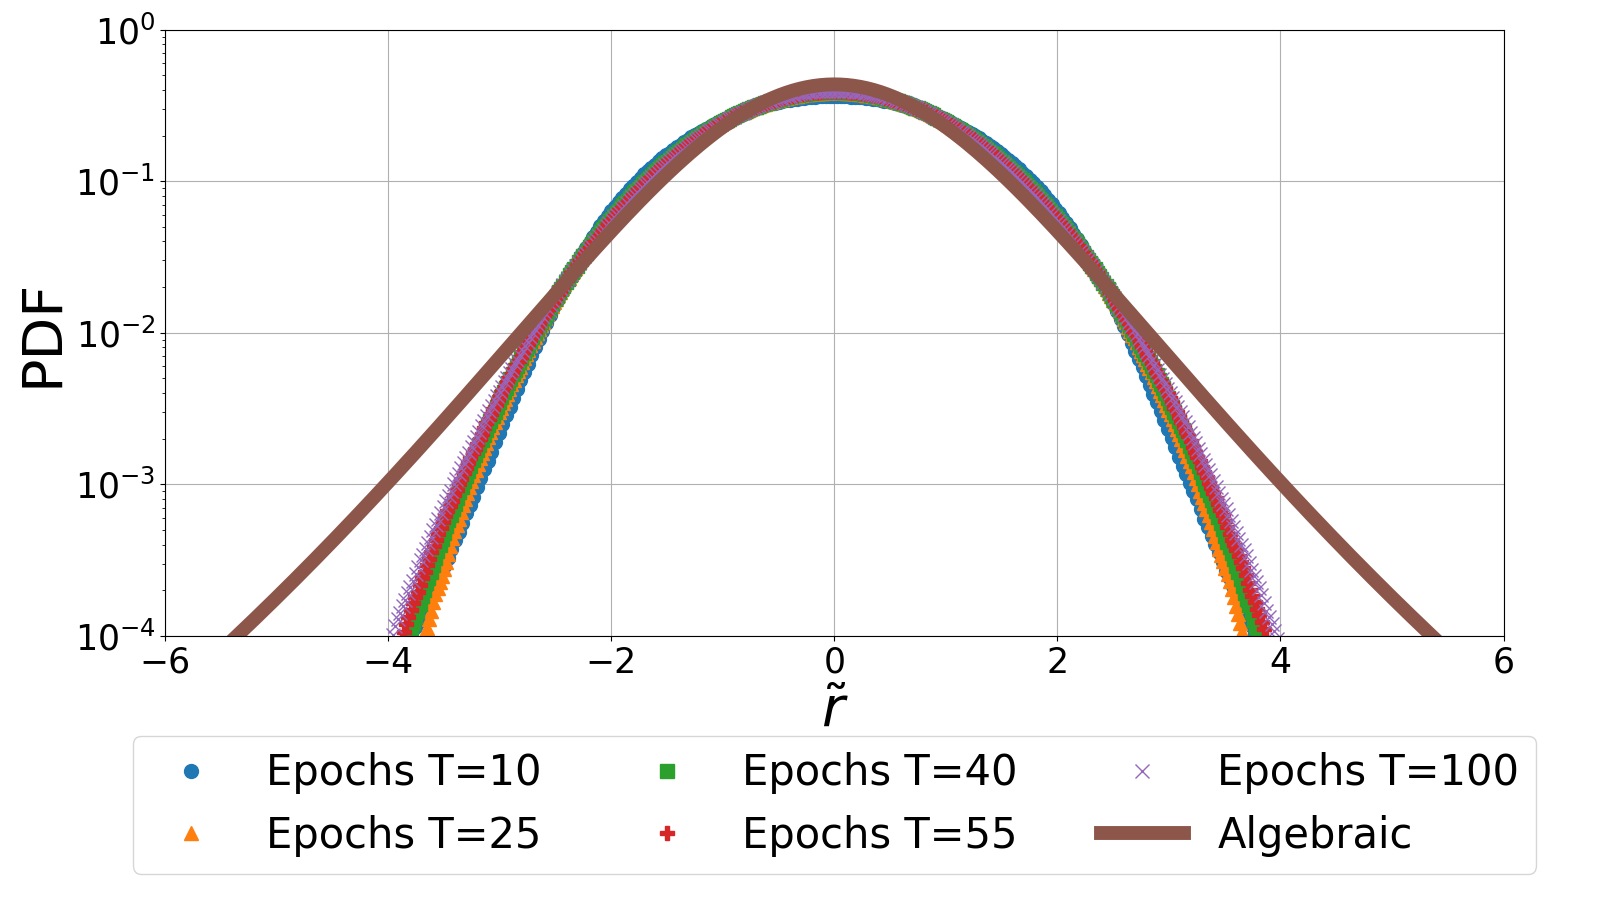
\includegraphics[width=0.6\columnwidth]
    {figures/06_epochs_sim_alg_ts_norm.png}
    \caption{Simulated aggregated rotated and scaled algebraic distributed
             returns ($\tilde{r}$) for fixed covariance and $K=200$ with
             normalization for the complete time series. $\Delta t = 1$ unit
             and epochs window lengths $T=10, 25, 40, 55, 100$ units.}
    \label{fig:epochs_alg_agg_ret_pairs_norm_full_ts}
\end{figure}

%%%%%%%%%%%%%%%%%%%%%%%%%%%%%%%%%%%%%%%%%%%%%%%%%%%%%%%%%%%%%%%%%%%%%%%%%%%%%%%
\subsection{Empirical results}
\label{subsec:emp_results}

After we found the problem in the method and solved for the simulated time
series, it is time to check the solution in the empirical data. We first
normalize the complete time series. Then we rotate and scale the returns and
finally we aggregate them. With this method, we can see how the ergodicity
defect disappears, as we expected from the simulations. Furthermore, we can now
see that with a epoch window length of $T = 25$ the returns show small fat
tails. Then, we confirm that the aggregated returns have internal structures
that we will use to define the exact multivariate amplitude distributions in
Sect. \ref{sec:exact_distributions}.

\begin{figure}[htbp]
    \centering
    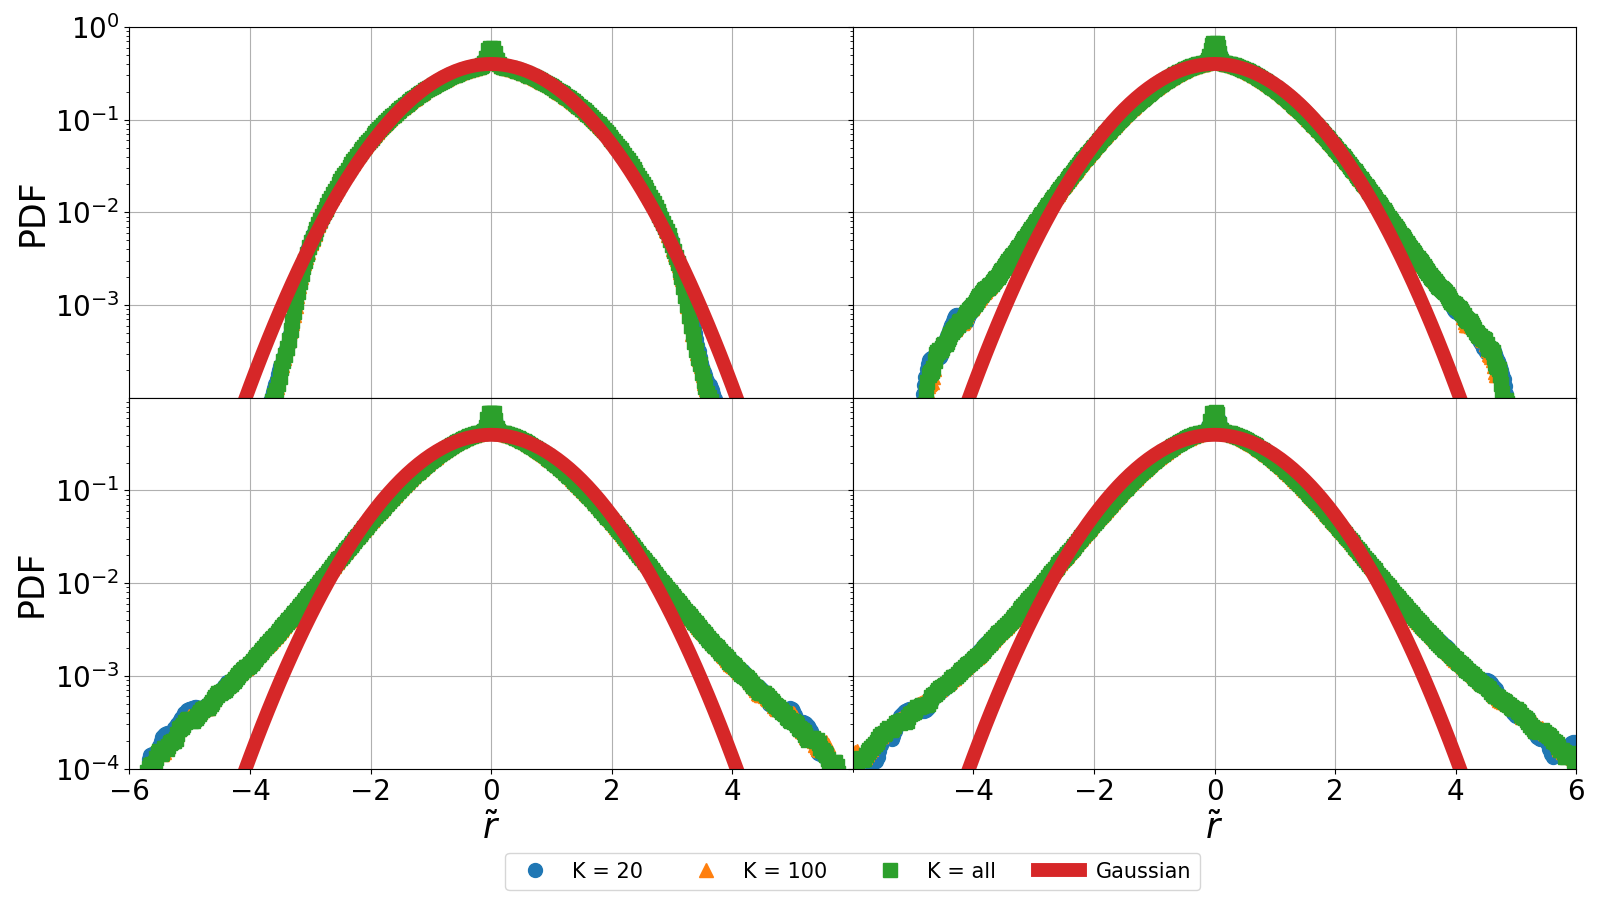
\includegraphics[width=0.8\columnwidth]
    {figures/06_window_comparison.png}
    \caption{Aggregated distribution of returns ($\tilde{r}$) for fixed
             covariance of different number of companies selected from the S\&P
             500 dataset. $\Delta t = 1d$ and different epochs window lengths
             $T=10d$ (top left), $T=25d$ (top right), $T=40d$ (bottom left) and
             $T=55d$ (bottom right).}
    \label{fig:window_comparison_long_norm}
\end{figure}